\documentclass[11pt]{article}

\usepackage[margin=1in]{geometry}
\usepackage{graphicx}
\usepackage{amsmath,amssymb}
\usepackage{booktabs}
\usepackage{array}
\usepackage{placeins}
\usepackage[numbers]{natbib}
\usepackage[colorlinks=true,allcolors=blue]{hyperref}
\usepackage{url}

\providecommand{\bibcommenthead}{}

\renewcommand{\contentsname}{Supplementary Contents}
\renewcommand{\thesection}{S\arabic{section}}
\renewcommand{\thefigure}{S\arabic{figure}}
\renewcommand{\thetable}{S\arabic{table}}
\numberwithin{equation}{section}
\renewcommand{\theequation}{\thesection.\arabic{equation}}

\title{Supplementary Information for\\
Risk-Aware Relational Spectral Recovery under Partial Quantum Observability}
\author{}
\date{}

\begin{document}
\maketitle
\tableofcontents

\section{Global constraint and clock-conditioned dynamics}

This note collects the background relational formulation used only in compressed
form in the main Methods. The total Hilbert space is written as
\begin{equation}
\mathcal{H}_{\mathrm{tot}}
=
\mathcal{H}_C\otimes \mathcal{H}_S,
\end{equation}
and physical states are taken to satisfy the global constraint
\begin{equation}
\hat H_{\mathrm{tot}}|\Psi\rangle=0.
\end{equation}
For a separable Hamiltonian
\begin{equation}
\hat H_{\mathrm{tot}}
=
\hat H_C\otimes I_S+I_C\otimes \hat H_S,
\end{equation}
a non-trivial product-basis solution requires matching clock and system energies,
\begin{equation}
\mathrm{Spec}(\hat H_C)\cap \mathrm{Spec}(-\hat H_S)\neq \emptyset .
\end{equation}
Indeed, in the product eigenbasis of $\hat H_C$ and $\hat H_S$, each component
has total energy $E^C_k+E^S_j$. A non-zero vector in the kernel can therefore have
support only on pairs satisfying $E^C_k=-E^S_j$. This is the finite-dimensional
version of the compatibility condition used in the simulations. It is not used in
the main text as an additional experimental assumption; it records why the
clock-system construction is internally consistent.

This condition is used as a consistency requirement for constructing finite
clock-system simulations; the main paper does not rely on a stronger claim that
the finite simulation realizes a complete theory of quantum time.

Clock labels are generated by the clock orbit
\begin{equation}
|\tau\rangle_C=e^{-i\hat H_C\tau}|0\rangle_C.
\end{equation}
Conditioning the global state on $|\tau\rangle_C$ gives
\begin{equation}
\rho_S(\tau)
=
\frac{
\operatorname{Tr}_C[
(|\tau\rangle\langle\tau|_C\otimes I_S)
|\Psi\rangle\langle\Psi|
]
}{
\operatorname{Tr}[
(|\tau\rangle\langle\tau|_C\otimes I_S)
|\Psi\rangle\langle\Psi|
]
}.
\end{equation}
All trajectories in the manuscript are ordered families over these internal clock
labels. They should not be read as externally time-parametrized histories.
The finite clock representation also imposes resolution limits. Neighboring clock
labels must be distinguishable enough to support separate conditional slices, but
the clock orbit remains finite and can recur. These effects are handled by using a
fixed ordered set of clock labels and by calibrating clock-consistency thresholds
from reference trajectories rather than asserting an ideal continuum clock.

The submitted implementation, retained only as an audit dataset, fixed the clock
object rather than tuning it per regime. The clock Hilbert space is one qubit,
the initial clock state is $|+\rangle_C$, and
\begin{equation}
H_C=0.8X_C .
\end{equation}
The sampled internal labels are
\begin{equation}
\tau_r\in\{-2.0,-1.5,-1.0,-0.5,0,0.5,1.0,1.5,2.0\},
\qquad m=9 .
\end{equation}
The same clock Hamiltonian, clock grid, and ordering convention are used for the
syndrome-first candidate, the relational candidate, the reference bank, and all
policy comparisons.

\section{Spectral deformation and detectability}

At each clock slice, the system state $\rho_S(\tau)$ is mapped to a weighted
relational graph with adjacency matrix $W^{(\tau)}$. The graph Laplacian is
\begin{equation}
L(\tau)=D^{(\tau)}-W^{(\tau)},
\qquad
D^{(\tau)}_{ii}=\sum_{j\neq i}W^{(\tau)}_{ij}.
\end{equation}
The graph functional is fixed by the code family in the reported experiments. For
the phase-flip repetition code, the edge weight is the absolute two-qubit
coherence
\begin{equation}
W_{ij}^{(\tau)}
=
\sum_{a\ne b}
\left|
\left(\rho_{ij}^{(\tau)}\right)_{ab}
\right|.
\end{equation}
For the bit-flip repetition code, the edge weight is the two-qubit mutual
information
\begin{equation}
W_{ij}^{(\tau)}
=
S(\rho_i^{(\tau)})
+S(\rho_j^{(\tau)})
-S(\rho_{ij}^{(\tau)}),
\end{equation}
where $S(\rho)=-\mathrm{Tr}(\rho\log\rho)$. Other relational functionals are
available in the codebase for diagnostics, but they are not mixed into the
reported $C_2$ versus $C_3^{\mathrm R}$ comparisons.
The code-dependent choice is fixed before policy evaluation and is not selected
per regime or per noise family.
We use the Laplacian spectrum rather than the density-matrix spectrum directly
because the decision variable is the collective connectivity pattern induced by
code-specific two-qubit relations, not the global eigenvalue distribution of the
state itself. Under a node relabeling the Laplacian changes only by permutation
similarity, so its spectrum summarizes relational structure without depending on
the arbitrary ordering of the three data qubits.
Noise and partial observation induce perturbations
\begin{equation}
L(\tau)\mapsto L(\tau)+\Delta L(\tau).
\end{equation}
If $\lambda_k(\tau)$ and $\tilde{\lambda}_k(\tau)$ denote the ordered spectra before
and after perturbation, Weyl-type perturbation control gives
\begin{equation}
|\tilde{\lambda}_k(\tau)-\lambda_k(\tau)|
\le
\|\Delta L(\tau)\|_2.
\end{equation}
This bound explains why the Laplacian spectrum is an appropriate diagnostic
object: perturbations in the relational graph create controlled spectral
deformations, and the trajectory-level distance accumulates those deformations
over clock labels. The experiments do not require every microscopic error to be
separately identifiable. They require only that the deformation relevant to the
recovery decision be large enough relative to calibrated background variation.

Consequently, non-trivial spectral deformations are detectable in principle when
they are resolved by the spectral estimator and exceed the calibrated background
variation. In the numerical implementation, this principle is used conservatively:
detection and recovery are judged by empirical trajectory distances, calibrated
admissibility penalties, and lower-tail recovery metrics rather than by a claim of
universal noise detectability.

\section{Relational trajectory-space formalism}

The clock-conditioned spectra define a spectral family
\begin{equation}
\Gamma_\Psi(\tau)=\Lambda(\tau)
=
(\lambda_1(\tau),\ldots,\lambda_n(\tau)).
\end{equation}
For sampled clock labels $\{\tau_r\}_{r=1}^m$, the computational distance between
two spectral families is
\begin{equation}
\begin{aligned}
d_{\mathcal M}^{ab}
&\equiv
d_{\mathcal M}(\Gamma^{(a)},\Gamma^{(b)}),\\
d_{\mathcal M}^{ab}
&=
\left(
\sum_{r=1}^{m}
w_r
\left\|
\Lambda^{(a)}(\tau_r)-\Lambda^{(b)}(\tau_r)
\right\|_2^2
\right)^{1/2}.
\end{aligned}
\end{equation}
We use the term relational spectral manifold only as a geometric shorthand for
this constrained metric trajectory space. The reported experiments use the
sampled spectra and the metric $d_{\mathcal M}$ directly. Differential-geometric
terms such as tangent vectors, geodesic curves, and Christoffel symbols are
therefore interpretive language, not assumptions required by the recovery
algorithm or by the policy validation. Boundary points, discrete reference banks,
and piecewise admissible regions are allowed in the computational formulation.

This is also why the construction is not an ordinary temporal smoother. A
standard smoother regularizes an externally ordered sequence. Here the ordering
comes from an internal clock-conditioned family, and the same candidate must
satisfy Laplacian validity, clock consistency, spectral smoothness, and
reference-anchor compatibility. The role of this section is therefore claim
calibration: it explains the metric object being audited without asserting a
foundational smooth-manifold theory.

\section{Admissibility penalties and recovery algorithm}

The admissible set is represented as an intersection of constraint families,
\begin{equation}
\mathcal{A}
=
\mathcal{A}_{\mathrm{lap}}
\cap
\mathcal{A}_{\mathrm{rel}}
\cap
\mathcal{A}_{\mathrm{ref}}.
\end{equation}
The implementation audits membership through four penalties. The Laplacian
penalty checks whether each slice remains a valid weighted-graph Laplacian:
\begin{align}
\Phi_{\mathrm{lap}}(\Gamma)
=
\sum_{r=1}^{m}
&
\Big(
\|L_r-L_r^\top\|_F^2
+\|L_r\mathbf 1\|_2^2
+\sum_k[-\lambda_k(L_r)]_+^2
\nonumber\\
&\quad
+\sum_{i\ne j}[L_{r,ij}]_+^2
+\left\|
\mathrm{diag}(L_r)+\sum_{j\ne i}L_{r,ij}
\right\|_2^2
\Big),
\end{align}
where $[x]_+=\max(x,0)$. The terms enforce symmetry, zero row sum,
positive-semidefinite spectrum, non-positive off-diagonal entries, and diagonal
consistency.

The smoothness penalty measures slice-to-slice spectral jumps:
\begin{equation}
\Phi_{\mathrm{smooth}}(\Gamma)
=
\sum_{r=1}^{m-1}
\frac{
\|\Lambda(\tau_{r+1})-\Lambda(\tau_r)\|_2^2
}{
(\tau_{r+1}-\tau_r)^2
}.
\end{equation}
The clock-consistency penalty makes a large spectral jump more severe when the
neighboring clock states are not well separated:
\begin{equation}
\Phi_{\mathrm{clock}}(\Gamma)
=
\sum_{r=1}^{m-1}
\frac{
\|\Lambda(\tau_{r+1})-\Lambda(\tau_r)\|_2
}{
1-|\langle\tau_r|\tau_{r+1}\rangle|^2+\epsilon
}.
\end{equation}
The reference-bank penalty is
\begin{equation}
\Phi_{\mathrm{ref}}(\Gamma)
=
\min_{\Gamma'\in\mathcal R}
d_{\mathcal M}(\Gamma,\Gamma')^2 .
\end{equation}

Thresholds are calibrated from reference trajectories as
\begin{equation}
\theta_k=\mu_k+\kappa\sigma_k,\qquad \kappa=1.5,
\end{equation}
with leave-one-out evaluation for the reference penalty so that a reference
trajectory does not calibrate its own distance to zero. For a candidate
$\Gamma_X$, the normalized violation used by the robust policy is
\begin{equation}
v_X
=
\max_k
\max\left\{0,\frac{\Phi_k(\Gamma_X)-\theta_k}{\theta_k+\epsilon}\right\}.
\end{equation}
The use of a maximum rather than an average is important for the robust policy.
Average violation can hide a single severe constraint failure, while the maximum
records the worst active excursion beyond threshold. This is the value denoted by
$v_A$ and $v_B$ in the $C_3^{\mathrm R}$ gate.

The reference bank contains three clean trajectories for each encoded code: the
logical reference state and two $\pm 20^\circ$ logical perturbations. These
reference trajectories use the same clock grid, clock Hamiltonian, and graph
functional as the observed row, but the noise channel is removed. The reference
anchor is selected only by trajectory distance:
\begin{equation}
\Gamma_{\mathrm{ref,anchor}}
=
\arg\min_{\Gamma'\in\mathcal R}
d_{\mathcal M}(\Gamma',\Gamma_{\mathrm{obs}})^2.
\end{equation}
No clean logical outcome, candidate fidelity, or oracle row label is used during
anchor selection. This separation is important because the reference anchor is
part of candidate construction, whereas fidelity and oracle quantities are held
out for evaluation.
The three-anchor bank is intentionally minimal. It is used to test whether a
small auditable reference family can support recovery-side control, not to
approximate a dense clean-state manifold.
The recovery objective is
\begin{align}
J_{\mathrm{rec}}(\Gamma)
=&
\alpha d_{\mathcal M}(\Gamma,\Gamma_{\mathrm{obs}})^2
+
\beta d_{\mathcal M}(\Gamma,\Gamma_{\mathrm{ref,anchor}})^2
\nonumber\\
&+
\lambda_1\Phi_{\mathrm{lap}}(\Gamma)
+
\lambda_2\Phi_{\mathrm{smooth}}(\Gamma)
+
\lambda_3\Phi_{\mathrm{clock}}(\Gamma).
\end{align}
The main experiments use the discrete admissible projection as the default
operator. A continuous convex refinement over local admissible combinations can be
used as a diagnostic extension, but it is not required for the main reported
policy results.
The reason is operational: the first-stage operator selects from a finite,
predeclared candidate set, so each accepted recovery can be traced to a reference
anchor, a recovery objective value, and a vector of admissibility violations. This
keeps the candidate construction separate from the downstream fidelity
evaluation and prevents the reported policy result from depending on hidden
continuous optimization flexibility.
The discrete projection stage evaluates a finite set of reference-compatible
candidate trajectories and selects the one minimizing the recovery objective while
respecting admissibility. If $\mathcal C_{\mathrm{ref}}$ is the finite
reference-compatible candidate set, the first-stage recovery is
\begin{equation}
\Gamma_1
=
\arg\min_{\Gamma\in\mathcal C_{\mathrm{ref}}}
J_{\mathrm{rec}}(\Gamma)
\quad
\mathrm{s.t.}\quad
\Phi_k(\Gamma)\le \theta_k\ \ \forall k .
\end{equation}
The optional refinement stage considers convex combinations of nearby admissible
candidates. For a local neighborhood
$\mathcal N_K(\Gamma_1)=\{\Gamma_j\}_{j=1}^{K}$, the feasible hull is
\begin{equation}
\mathcal H_K(\Gamma_1)
=
\left\{
\sum_{j=1}^{K}\alpha_j\Gamma_j:
\alpha_j\ge 0,\ 
\sum_{j=1}^{K}\alpha_j=1
\right\}.
\end{equation}
The diagnostic second-stage candidate is then
\begin{equation}
\Gamma_2
=
\arg\min_{\Gamma\in\mathcal H_K(\Gamma_1)}
J_{\mathrm{rec}}(\Gamma)
\quad
\mathrm{s.t.}\quad
\Phi_k(\Gamma)\le \theta_k\ \ \forall k .
\end{equation}
The reported C3R policy comparisons use the conservative application rule
\begin{equation}
\Gamma_{\mathrm{rec}}=\Gamma_1,
\end{equation}
while $\Gamma_2$ is retained only for sensitivity diagnostics. This two-stage
design keeps the paper-facing operator auditable while leaving room for continuous
diagnostics. In particular, it avoids post-hoc candidate shaping, preserves
row-level interpretability, and makes the intervention metrics attributable to
the policy gate rather than to an additional refinement step. Stage 2 is therefore
reported as a diagnostic stress test of the recovery geometry, not as a second
source of final-policy performance.

\section{Encoded-QEC simulation protocol}

The encoded-QEC testbed uses three-qubit repetition codes in bit-flip and
phase-flip configurations. Noise families include bit-flip, phase-flip,
depolarizing, dephasing, and mixed-Pauli channels. Each simulation row constructs
two candidates:
\begin{equation}
A=\text{syndrome-first decoded recovery},
\qquad
B=\text{relational admissible recovery}.
\end{equation}
Candidate $A$ is the conventional decoder-facing baseline. Candidate $B$ is the
output of admissible spectral recovery. The policy layer never changes the
candidate construction; it only decides which candidate to trust on each row.
This design isolates policy behavior. If the candidates themselves changed across
partial, noisy, or ambiguous syndrome protocols, it would be difficult to tell
whether an observed improvement came from better recovery construction or from a
better decision rule. Here the decision layer is tested against a fixed pair of
candidate recoveries, while syndrome observability affects the policy evidence and
uncertainty diagnostics.

Syndrome observability is controlled by an observation ratio, syndrome-bit noise,
ambiguity, measurement error, reset error, and measured information loss. The
uncertainty proxy used by the robust gate is
\begin{equation}
u_{\mathrm{raw}}
=
(1-r_{\mathrm{obs}})
+p_{\mathrm{noise}}
+a_{\mathrm{amb}}
+p_{\mathrm{meas}}
+p_{\mathrm{reset}}
+\ell_{\mathrm{syn}},
\qquad
u_{\mathrm{syn}}=\mathrm{clip}_{[0,1]}(u_{\mathrm{raw}}).
\end{equation}
Figures~\ref{fig:supp-qec-encoders} and~\ref{fig:supp-qec-recovery} show the
explicit circuit-level implementation of the testbed. The encoder circuits draw
the three-qubit repetition-code conventions: bit-flip protection uses two CNOTs
from the data qubit $q_0$ to $q_1$ and $q_2$, while phase-flip protection appends
Hadamards on all three qubits to map the bit-flip stabilizers into the $X$ basis.
The recovery circuits draw the corresponding syndrome-extraction circuits with
two ancillas $a_0,a_1$ measured into classical bits $s_0,s_1$ and feed-forward
$X$ corrections gated on the syndrome values
$\{0\text{x}1,0\text{x}2,0\text{x}3\}$. The
clock-conditioned data state $\rho_{\mathrm{data}}(\tau)$ is injected on
$\{q_0,q_1,q_2\}$ at each clock slice; the relational graph functional above is
computed from this injected state before any syndrome operation.
The stress protocols used in the main analysis are clean syndrome, partial
syndrome, noisy syndrome, partial-plus-noisy syndrome, and ambiguity with
measurement/reset errors.
The clean map identifies operating zones when direct syndrome information is
reliable. The partial and partial-plus-noisy maps test missing evidence and
combined degradation. The noisy-only map tests random syndrome-bit corruption
without reducing observation ratio. The ambiguity-plus-measurement map tests
whether uncertainty due to ambiguous or physically corrupted syndrome evidence
produces the same risk-control behavior.

\begin{figure}[t]
\centering
\begin{minipage}{0.47\textwidth}
\centering
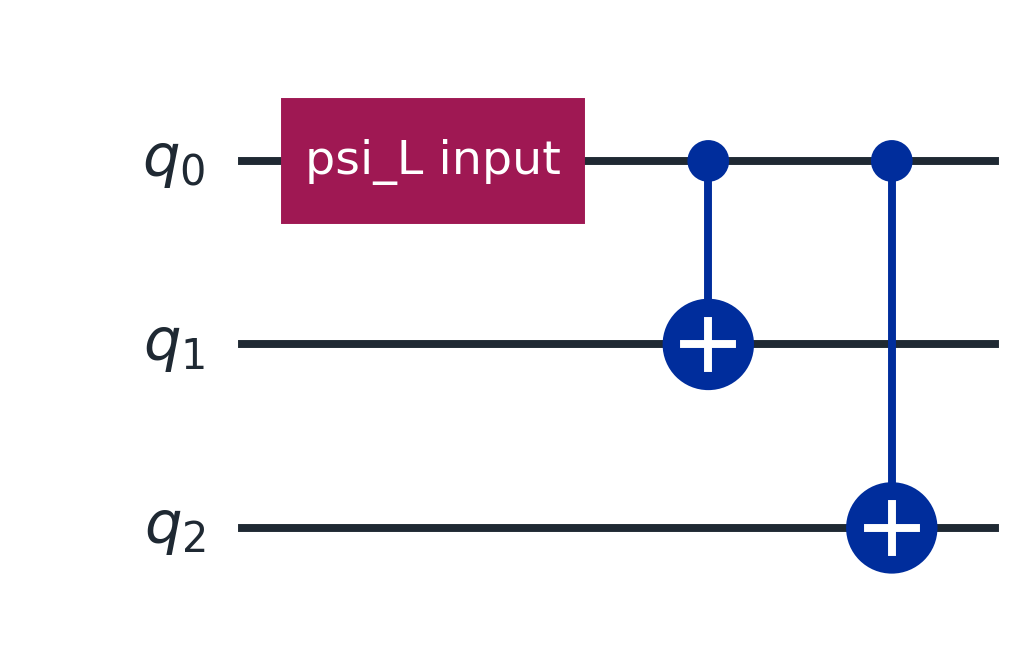
\includegraphics[width=\linewidth]{figs/supplementary_circuits/supp_bitflip_encoding.png}
\end{minipage}
\hfill
\begin{minipage}{0.47\textwidth}
\centering
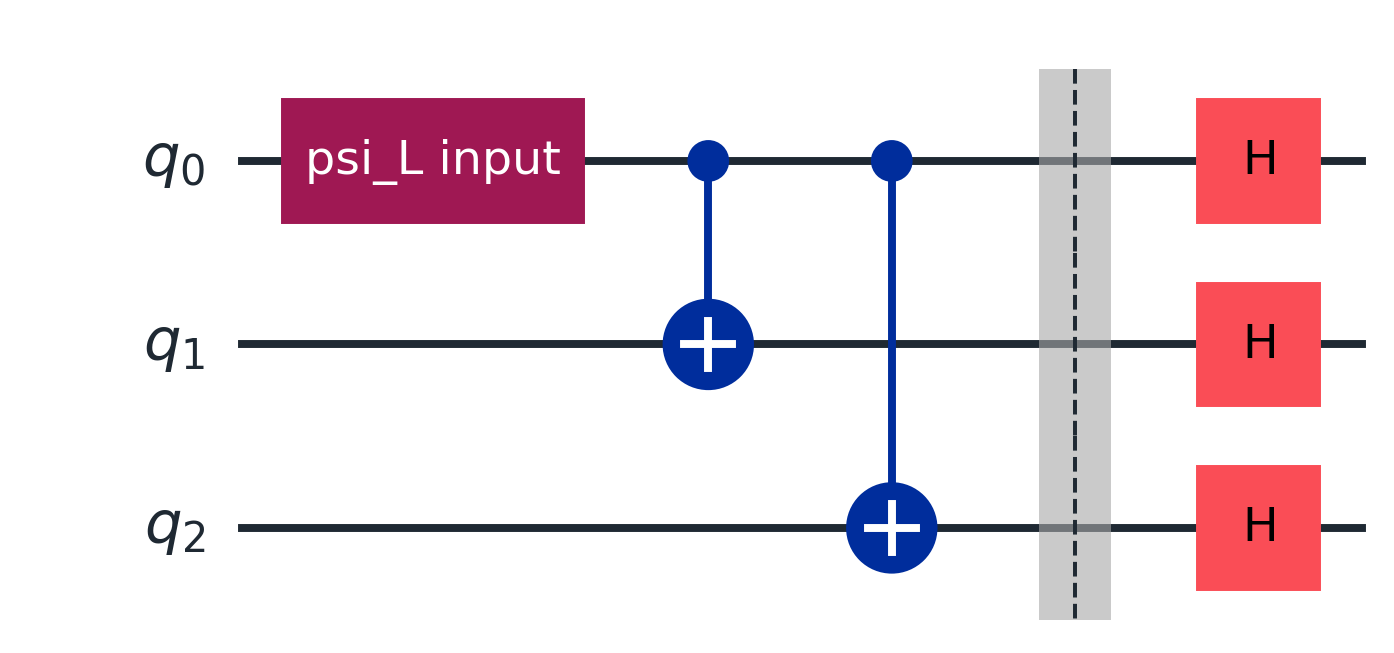
\includegraphics[width=\linewidth]{figs/supplementary_circuits/supp_phaseflip_encoding.png}
\end{minipage}
\caption{Encoder schematics for the encoded-QEC testbed. The left panel shows
the bit-flip repetition-code encoder and the right panel shows the phase-flip
encoder obtained by adding Hadamards on all three data qubits. The label
$\psi_L$ denotes the logical input state used to initialize the repetition-code
block.}
\label{fig:supp-qec-encoders}
\end{figure}

\begin{figure}[t]
\centering
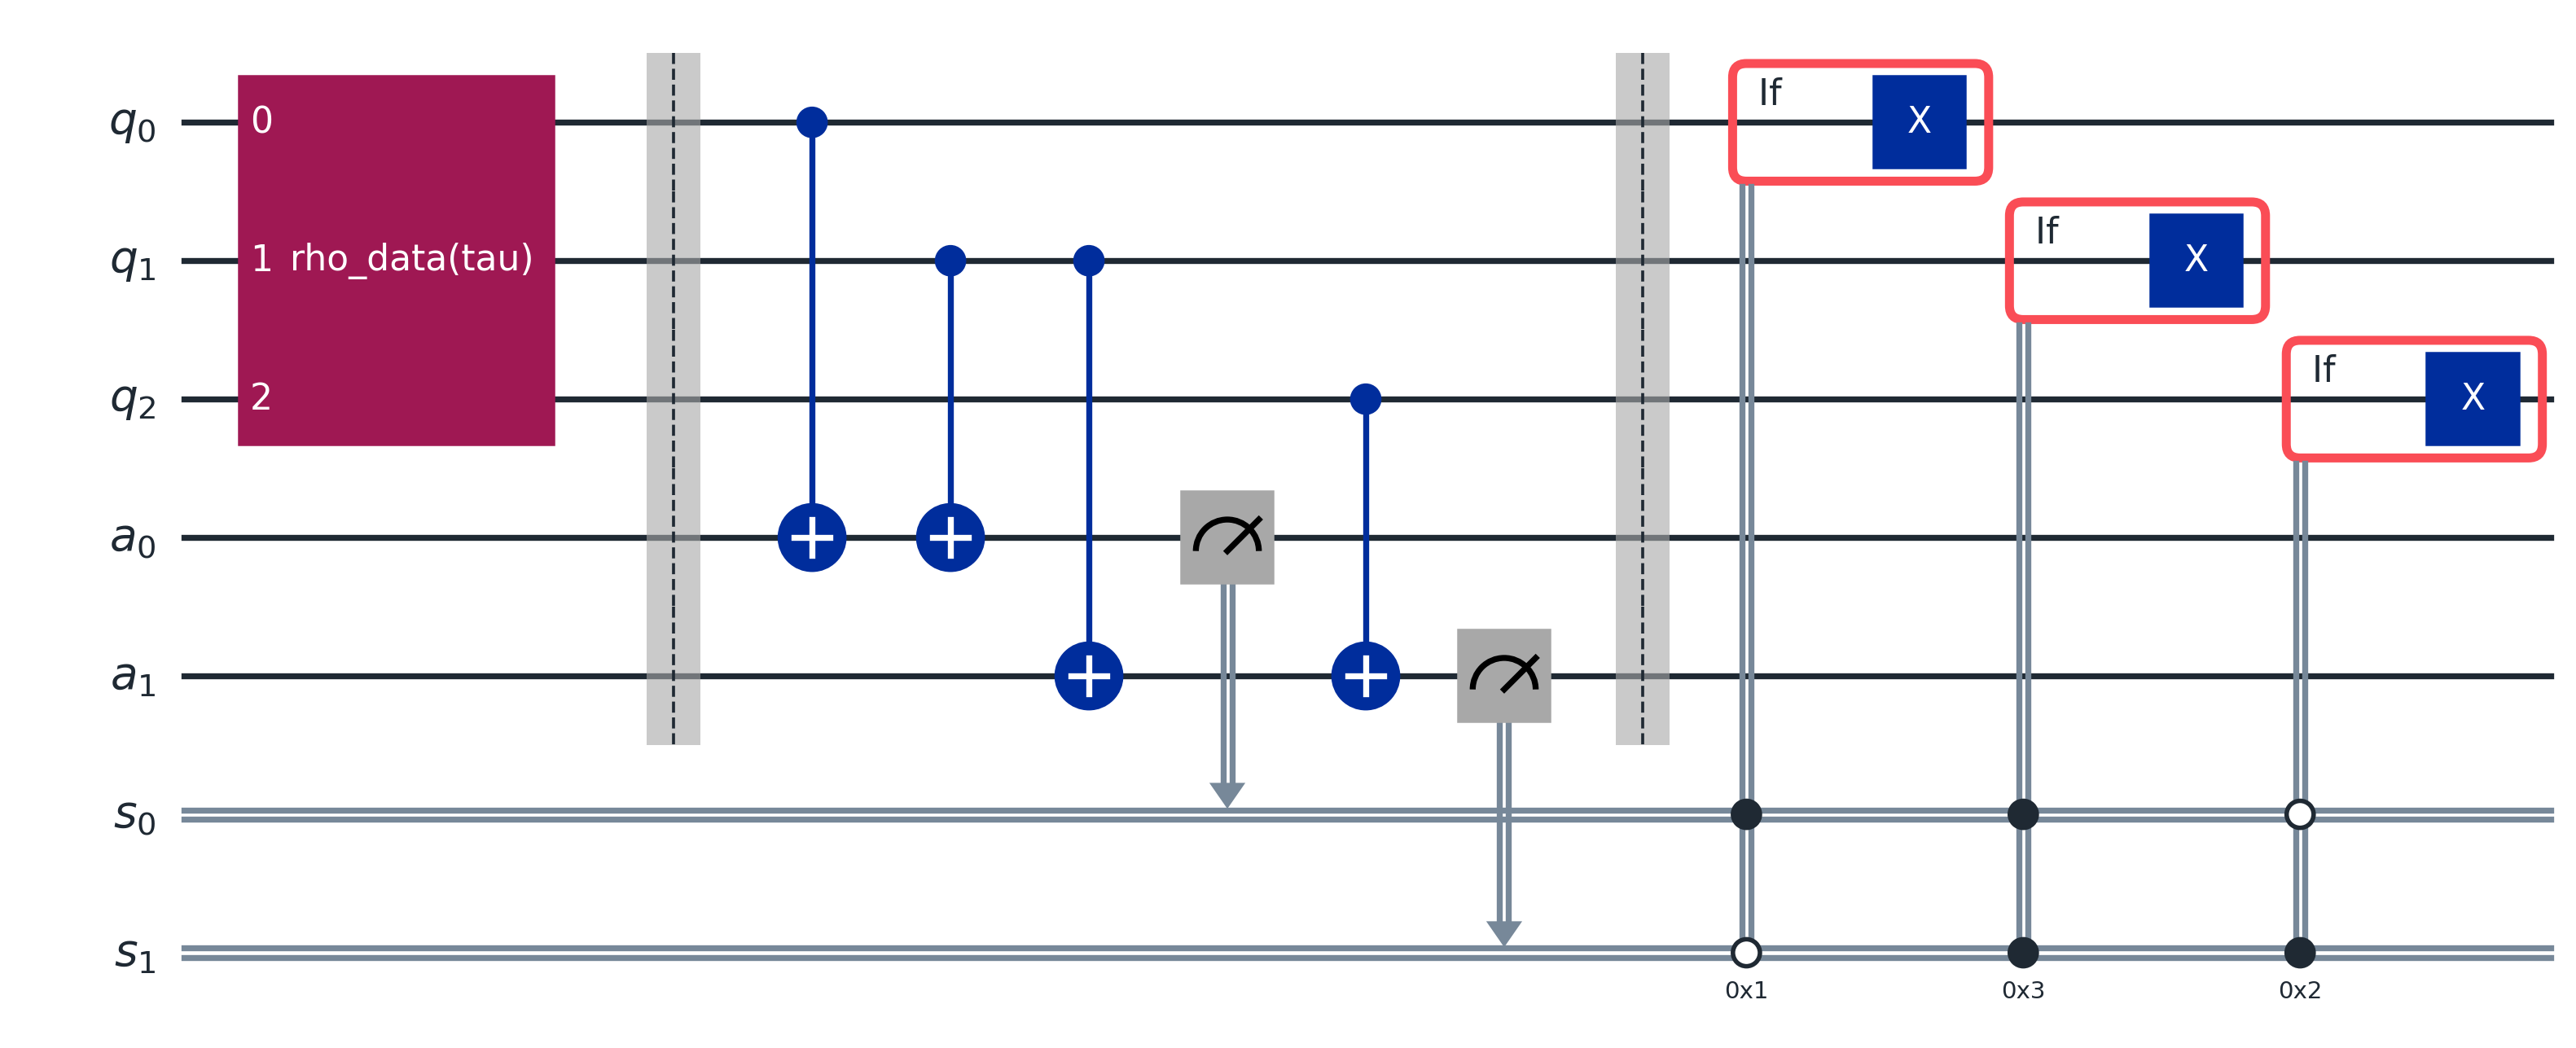
\includegraphics[width=\textwidth]{figs/supplementary_circuits/supp_bitflip_syndrome_recovery.png}
\vspace{0.75em}

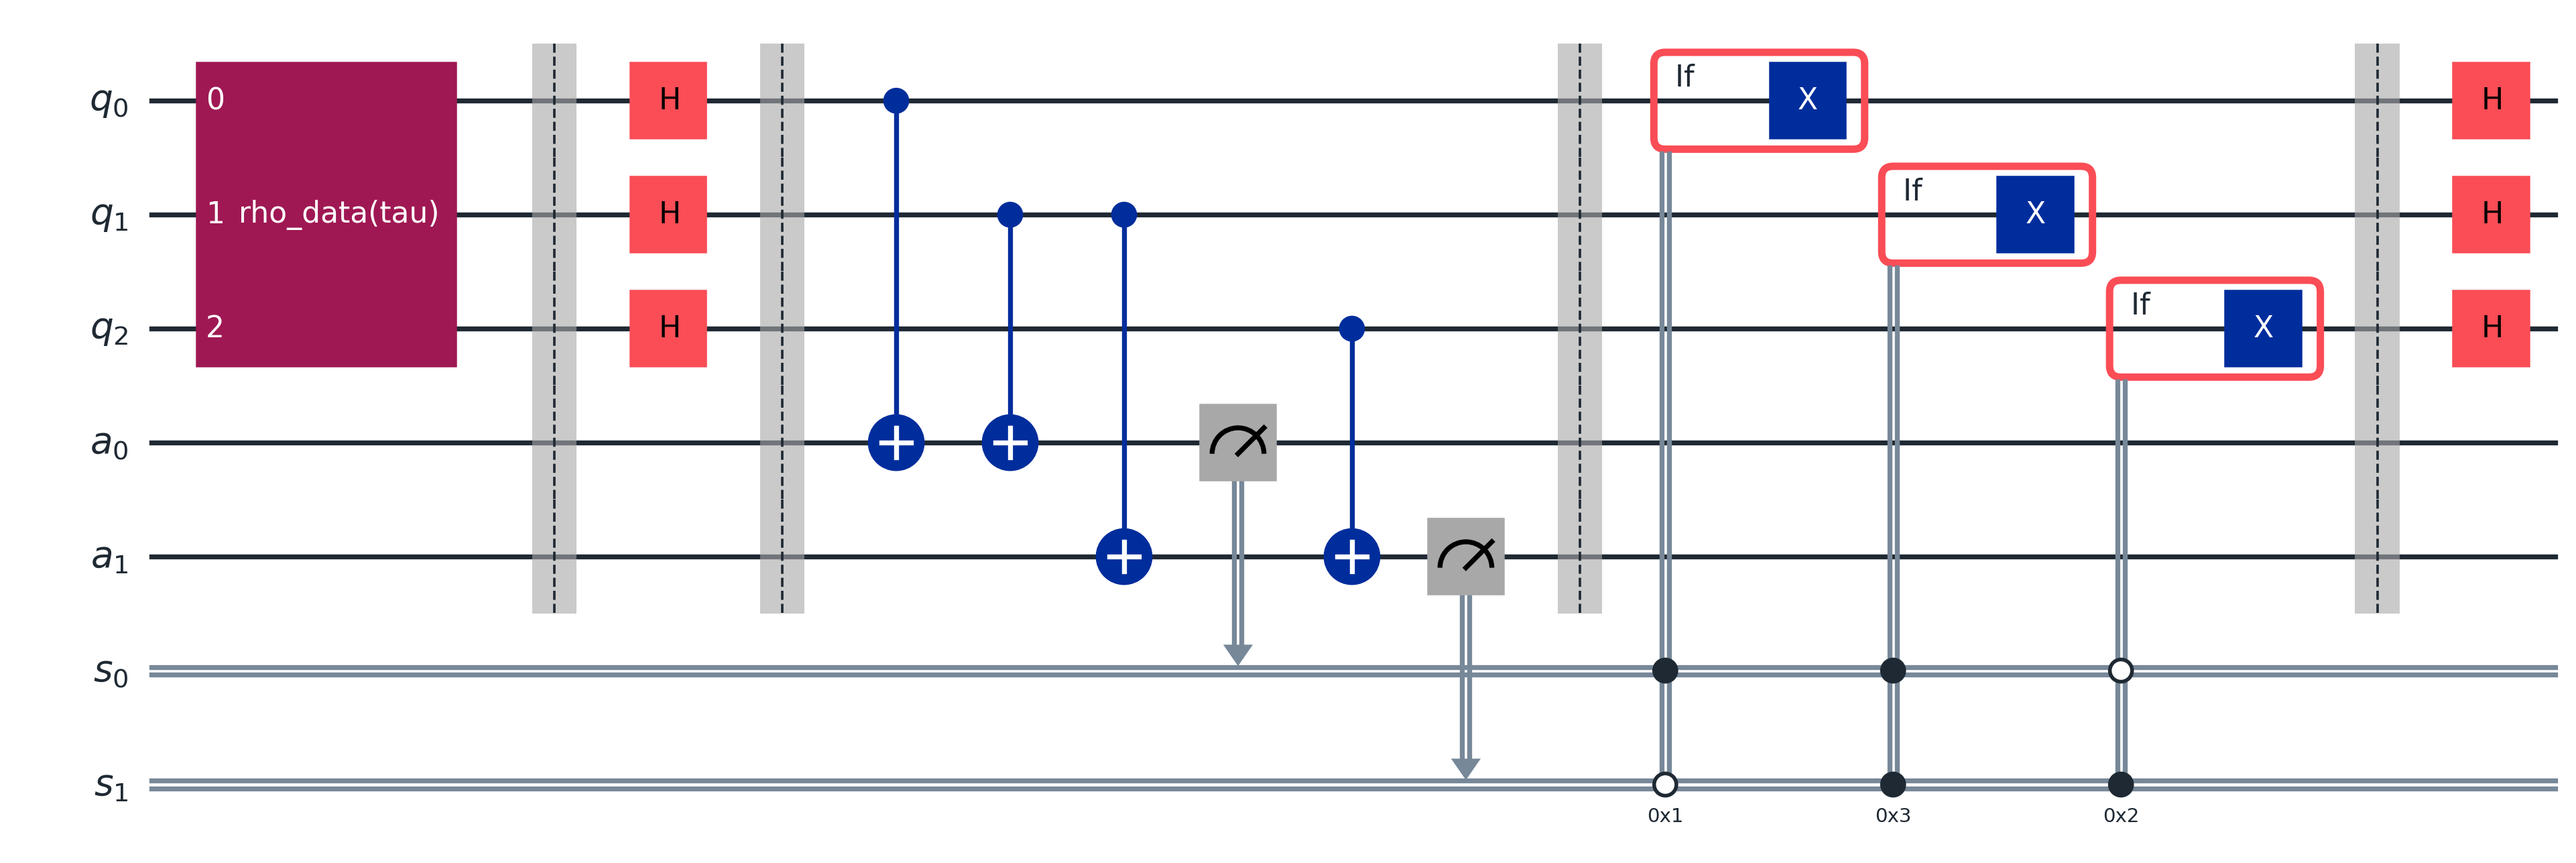
\includegraphics[width=\textwidth]{figs/supplementary_circuits/supp_phaseflip_syndrome_recovery.png}
\caption{Syndrome-extraction and feed-forward recovery schematics. The upper
panel shows the bit-flip recovery circuit and the lower panel shows the
phase-flip recovery circuit. The state $\rho_{\mathrm{data}}(\tau)$ denotes the
clock-conditioned three-qubit data-register state injected before syndrome
extraction. Ancillas $a_0,a_1$ store the two parity checks and are measured into
the classical register $s_0,s_1$, with $s_0$ the least significant bit. The
feed-forward integer convention is therefore $s_1s_0$: $0\text{x}1=01$ applies
$X$ to $q_0$, $0\text{x}3=11$ applies $X$ to $q_1$, and $0\text{x}2=10$ applies
$X$ to $q_2$. For the phase-flip circuit, Hadamards before and after syndrome
extraction move the same correction logic into the phase-flip protection basis.
The simulations trace out the ancilla register after recovery; the schematic is
drawn in system-qubit order $q_0,q_1,q_2$.}
\label{fig:supp-qec-recovery}
\end{figure}

\section{Policy maps and operating-zone analysis}

The four policies compared in the manuscript are deterministic maps from the same
two candidates to one selected recovery. $C_1$ is the conservative rule-based
hybrid. $C_2$ is the balanced proposal policy with score
\begin{equation}
S_X^{(2)}
=
\lambda_s s_X
-\lambda_t d_X
-\lambda_i(1-a_X)
+\lambda_o\frac{1}{1+J_X}.
\end{equation}
$C_3$ is a hard-admissibility ablation: it selects the uniquely admissible
candidate when exactly one candidate is admissible, and otherwise uses a
safety-weighted score. The clean-regime result that $C_3$ does not form an
independent operating zone is interpreted as an ablation result, not as the central
claim of the paper.
The reason for retaining $C_3$ is methodological. It tests the simpler hypothesis
that strict admissibility alone is enough to create a useful safety-first region.
The negative operating-zone result indicates that this Boolean criterion is too
coarse once inadmissibility has already been priced into the balanced score used
by $C_2$. This motivates the one-sided veto design of $C_3^{\mathrm R}$.

The revised policy $C_3^{\mathrm R}$ treats $C_2$ as a proposal and applies a
one-sided veto:
\begin{equation}
C_3^{\mathrm R}=B
\Longleftrightarrow
[C_2=B]
\wedge[\Delta S\ge\delta_S]
\wedge[v_A\ge\delta_A]
\wedge[B\ \mathrm{admissible},\,v_B\le\delta_B]
\wedge[u_{\mathrm{syn}}\le u_{\max}].
\end{equation}
The main operating point is
\begin{equation}
\delta_S=0,\qquad
\delta_A=0,\qquad
\delta_B=0,\qquad
u_{\max}=0.99.
\end{equation}
Thus
\begin{equation}
C_3^{\mathrm R}=B\Rightarrow C_2=B,
\end{equation}
so the revised controller can block proposed relational switches but cannot create
new ones.
The useful diagnostics for $C_3^{\mathrm R}$ are therefore conditional on $C_2$
proposing $B$. Unconditional switch rates can be misleading because most rows may
already be preserved by $C_2$. The intervention analysis in the main text and
result tables consequently report block rate given $C_2=B$, harmful-block
precision, harmful-switch recall, beneficial-switch block rate, and net
intervention effect.  Beneficial-switch retention is the complementary quantity.

\begin{table}[ht]
\centering
\scriptsize
\caption{Clean-regime preferred-policy counts over the 240-cell operating map.
Each cell is averaged over ten random seeds.}
\label{tab:supp-clean-policy-counts}
\begin{tabular}{@{}lrrl@{}}
\toprule
Policy & Cells & Share & Interpretation \\
\midrule
$C_1$ & 197 & 0.8208 & Default conservative hybrid region. \\
$C_2$ & 43 & 0.1792 & Structured correction region; all cells are phase-flip code rows. \\
$C_3$ & 0 & 0.0000 & No independent strict-admissibility zone. \\
$C_3^{\mathrm R}$ & 0 & 0.0000 & No clean-regime veto trigger at the default gate. \\
\bottomrule
\end{tabular}
\end{table}

\begin{table}[ht]
\centering
\scriptsize
\caption{Noise-family composition of the clean $C_2$ preferred region.}
\label{tab:supp-clean-noise-composition}
\begin{tabular}{@{}lr@{}}
\toprule
Noise family & $C_2$-preferred cells \\
\midrule
Bit flip & 2 \\
Dephasing & 16 \\
Depolarizing & 6 \\
Mixed Pauli & 9 \\
Phase flip & 10 \\
\bottomrule
\end{tabular}
\end{table}

\begin{table}[ht]
\centering
\scriptsize
\caption{Partial-syndrome preferred-policy counts by observed syndrome ratio.}
\label{tab:supp-partial-by-robs}
\begin{tabular}{@{}lrrrrr@{}}
\toprule
$r_{\mathrm{obs}}$ & Cells & $C_1$ & $C_2$ & $C_3$ & $C_3^{\mathrm R}$ \\
\midrule
1.00 & 72 & 37 & 35 & 0 & 0 \\
0.75 & 72 & 72 & 0 & 0 & 0 \\
0.50 & 72 & 12 & 0 & 0 & 60 \\
0.25 & 72 & 14 & 0 & 0 & 58 \\
\bottomrule
\end{tabular}
\end{table}

\begin{table}[ht]
\centering
\scriptsize
\caption{Noisy-only preferred-policy counts by syndrome-bit noise probability.
The robust policy remains inactive in this negative-control map.}
\label{tab:supp-noisy-by-pnoise}
\begin{tabular}{@{}lrrrrr@{}}
\toprule
$p_{\mathrm{noise}}$ & Cells & $C_1$ & $C_2$ & $C_3$ & $C_3^{\mathrm R}$ \\
\midrule
0.00 & 72 & 37 & 35 & 0 & 0 \\
0.01 & 72 & 49 & 23 & 0 & 0 \\
0.03 & 72 & 51 & 21 & 0 & 0 \\
0.05 & 72 & 51 & 21 & 0 & 0 \\
0.10 & 72 & 61 & 11 & 0 & 0 \\
\bottomrule
\end{tabular}
\end{table}

\begin{table}[ht]
\centering
\scriptsize
\caption{Representative partial-plus-noisy policy-map rows showing regime cells
where $C_3^{\mathrm R}$ is the preferred policy. Each row contains 72 cells.}
\label{tab:supp-partial-noisy-active}
\begin{tabular}{@{}ccrrrr@{}}
\toprule
$r_{\mathrm{obs}}$ & $p_{\mathrm{noise}}$ & $C_1$ & $C_2$ & $C_3$ & $C_3^{\mathrm R}$ \\
\midrule
0.50 & 0.03 & 13 & 0 & 0 & 59 \\
0.50 & 0.05 & 12 & 0 & 0 & 60 \\
0.50 & 0.10 & 15 & 0 & 0 & 57 \\
\bottomrule
\end{tabular}
\end{table}

\FloatBarrier

\section{Metric definitions}

Let $\Delta F_C$ be the logical-fidelity gain of policy $C$. The false-safe and
success thresholds are fixed before policy comparison:
\begin{equation}
\varepsilon_F=0.01,\qquad F_{\mathrm{success}}=0.99 .
\end{equation}
Central performance is summarized by mean gain, logical-success rate
\begin{equation}
P[F_C\ge F_{\mathrm{success}}],
\end{equation}
and non-worsening rate
\begin{equation}
P[\Delta F_C\ge 0].
\end{equation}
Downside risk is summarized by false-safe fidelity rate,
\begin{equation}
\mathrm{FS}_F(C)=P[\Delta F_C<-\varepsilon_F],
\end{equation}
the lower quantile $q_{0.05}(C)$, and
\begin{equation}
\mathrm{CVaR}_{0.05}(C)
=
\operatorname{E}_{\mathrm{emp}}[\Delta F_C\mid \Delta F_C\le q_{0.05}(C)].
\end{equation}

For $C_3^{\mathrm R}$, the intervention metrics are conditional on $C_2$ proposing
$B$. The block indicator is
\begin{equation}
B_R=\mathbf{1}[C_2=B]\mathbf{1}[C_3^{\mathrm R}=A].
\end{equation}
Harmful and beneficial proposed switches are
\begin{equation}
H_2=\mathbf{1}[C_2=B]\mathbf{1}[\Delta F_A>\Delta F_B+\varepsilon_F],
\end{equation}
\begin{equation}
G_2=\mathbf{1}[C_2=B]\mathbf{1}[\Delta F_B>\Delta F_A+\varepsilon_F].
\end{equation}
We report block rate, harmful-block precision, harmful-switch recall,
beneficial-switch block rate, prevented loss, missed gain, and net intervention
effect.  Beneficial-switch retention is one minus the beneficial-switch block
rate. The uncertainty-bin analysis groups rows by $u_{\mathrm{raw}}$ to check
whether the robust policy behaves as an uncertainty-conditioned intervention rather
than as an unconditional score adjustment.
The scalar net intervention effect is
\begin{equation}
E_{\mathrm{net}}
=
\sum_i B_{R,i}(\Delta F_{A,i}-\Delta F_{B,i}),
\end{equation}
equivalently,
\begin{equation}
E_{\mathrm{net}}
=
\sum_i B_{R,i}\max\{0,\Delta F_{A,i}-\Delta F_{B,i}\}
-
\sum_i B_{R,i}\max\{0,\Delta F_{B,i}-\Delta F_{A,i}\}.
\end{equation}
Thus the same scalar can be read as prevented harmful-switch loss minus missed
beneficial-switch gain. A positive value means that blocked switches improved
aggregate fidelity relative to accepting the $C_2$ proposal. We also report
$E_{\mathrm{net}}/\sum_i B_{R,i}$ and
$E_{\mathrm{net}}/\sum_i\mathbf{1}[C_{2,i}=B]$ to separate aggregate benefit from
the number of vetoed proposals.
For offline comparison we also compute oracle regret,
\begin{equation}
\Delta F^\star=\max\{\Delta F_A,\Delta F_B\},
\qquad
\mathrm{Reg}(C)=\Delta F^\star-\Delta F_C.
\end{equation}
The oracle is not available to the policy; it is used only to quantify how far the
chosen candidate is from the best candidate available on that simulation row. This
diagnostic is especially useful when mean gain and false-safe rate point in
different directions.

\section{Threshold and uncertainty diagnostics}

This section audits the two threshold choices that could otherwise appear
arbitrary: the uncertainty gate $u_{\max}$ in the robust policy and the
admissibility calibration factor $\kappa$. The purpose is not to tune an optimum
threshold after seeing the outcomes, but to show how the reported operating point
behaves relative to nearby counterfactual settings and negative controls.

The default robust gate uses $u_{\max}=0.99$. This value should not be interpreted
as a calibrated posterior confidence level. It is a saturation guard for the
additive stress index $u_{\mathrm{raw}}$ after clipping. Table~\ref{tab:umax-sens}
reports offline counterfactuals for the same rows under alternative
$u_{\max}$ values.

\begin{table}[ht]
\centering
\scriptsize
\setlength{\tabcolsep}{3pt}
\caption{$C_3^{\mathrm R}$ uncertainty-threshold sensitivity. Mean gain and false-safe fidelity
rate are recomputed from the same result rows after changing only the
$u_{\max}$ gate. Noisy-only is included as a negative control; $u_{\max}$ has no
effect there because no row triggers the robust gate.}
\label{tab:umax-sens}
\begin{tabular}{@{}lcrrrrrr@{}}
\toprule
Regime & $u_{\max}$ & mean gain & $\mathrm{FS}_F$ & blocked &
precision & ben. block & net/block \\
\midrule
Noisy-only & any & 0.1169 & 0.0678 & 0 & -- & -- & -- \\
\midrule
Partial & 0.75 & 0.1189 & 0.0340 & 543 & 0.8508 & 0.4833 & 0.0106 \\
Partial & 0.99 & 0.1189 & 0.0389 & 476 & 0.8697 & 0.3750 & 0.0119 \\
Partial & 1.00 & 0.1169 & 0.0694 & 0 & -- & -- & -- \\
Partial+noisy & 0.75 & 0.1205 & 0.0000 & 821 & 0.8465 & 1.0000 & 0.0092 \\
Partial+noisy & 0.99 & 0.1212 & 0.0134 & 670 & 0.8791 & 0.6739 & 0.0136 \\
Partial+noisy & 1.00 & 0.1170 & 0.0685 & 0 & -- & -- & -- \\
Ambig.+meas. & 0.75 & 0.1608 & 0.0000 & 480 & 0.7896 & 0.5316 & 0.0061 \\
Ambig.+meas. & 0.99 & 0.1604 & 0.0000 & 357 & 0.7759 & 0.4211 & 0.0044 \\
Ambig.+meas. & 1.00 & 0.1600 & 0.0000 & 0 & -- & -- & -- \\
\bottomrule
\end{tabular}
\end{table}

For historical implementation documentation, the admissibility thresholds contain
the calibration constant $\kappa$ in
$\theta_k=\mu_k+\kappa\sigma_k$. To check that the default $\kappa=1.5$ is not a
single-point artifact, we ran the recovery-ablation sweep with
$\kappa\in\{1.0,1.5,2.0\}$ while holding the noise families, noise strengths, and
reference-bank widths fixed. The sweep covers bit-flip, phase-flip, and dephasing
stress scenarios at five strengths and three bank widths, giving 45 cases per
calibration point.

\begin{table}[ht]
\centering
\scriptsize
\setlength{\tabcolsep}{4pt}
\caption{Historical calibration-sweep sensitivity for the submitted recovery objective.
Recovered admissible is the calibrated-admissibility rate of the final recovered
trajectory. Candidate improvement is the rate at which the optional Stage-2
admissible candidate improves the recovery objective relative to Stage 1, and
helpful tradeoff additionally requires non-worse clean distance.}
\label{tab:kappa-sens}
\begin{tabular}{@{}rrrrrr@{}}
\toprule
$\kappa$ & cases & rec. admiss. & cand. improve &
mean cand. $\Delta J$ & helpful \\
\midrule
1.0 & 45 & 0.2000 & 0.5556 & -0.1100 & 0.1111 \\
1.5 & 45 & 1.0000 & 0.6667 & 0.1702 & 0.1111 \\
2.0 & 45 & 1.0000 & 0.6667 & 0.1702 & 0.1111 \\
\bottomrule
\end{tabular}
\end{table}

The default $\kappa=1.5$ is on the same plateau as $\kappa=2.0$ in this sweep,
whereas the stricter $\kappa=1.0$ calibration sharply reduces recovered
admissibility and gives a negative mean candidate objective gain. The helpful
tradeoff rate is invariant across $\kappa$ in this sweep, indicating that these
$\kappa$ changes affect admissibility coverage and Stage-2 candidate acceptance
more than the underlying clean-distance behavior. This supports using
$\kappa=1.5$ as a historical implementation tolerance, but it does not identify
a discriminative admissibility gate on the submitted main grid: candidate $B$ is
admissible in every row. No Stage-2 refinements were accepted by the conservative
application rule in this sweep, so Table~\ref{tab:kappa-sens} is retained as
calibration documentation rather than policy-performance evidence.

\begin{table}[ht]
\centering
\scriptsize
\setlength{\tabcolsep}{3pt}
\caption{Uncertainty-bin intervention summary at the default $u_{\max}=0.99$.
Bins with zero blocks show that the gate is concentrated near saturated syndrome
stress rather than acting as an unconditional score penalty.}
\label{tab:uncertainty-bin}
\begin{tabular}{@{}llrrrrrr@{}}
\toprule
Regime & $u_{\mathrm{raw}}$ bin & cases & $C_2=B$ & blocked &
block rate & precision & net \\
\midrule
Partial & $<1.00$ & 1638 & 618 & 0 & 0.0000 & -- & 0.0000 \\
Partial & $[1,\infty)$ & 1242 & 476 & 476 & 1.0000 & 0.8697 & 5.6616 \\
Partial+noisy & $[0.75,1.00)$ & 516 & 180 & 29 & 0.1611 & 0.6897 & -0.3097 \\
Partial+noisy & $[1,\infty)$ & 1644 & 641 & 641 & 1.0000 & 0.8877 & 9.4309 \\
Ambig.+meas. & $<1.00$ & 2142 & 538 & 0 & 0.0000 & -- & 0.0000 \\
Ambig.+meas. & $[1,\infty)$ & 1458 & 357 & 357 & 1.0000 & 0.7759 & 1.5749 \\
\bottomrule
\end{tabular}
\end{table}

These diagnostics show that the default $u_{\max}=0.99$ gate behaves primarily as
a saturation guard. When $u_{\max}=1.00$, the veto is disabled in the reported
degraded regimes and $C_3^{\mathrm R}$ collapses to $C_2$. When
$u_{\max}=0.75$, the controller becomes more conservative, reducing false-safe
failures further in some regimes but increasing beneficial-switch loss. The
negative net value in the partial-plus-noisy $[0.75,1.00)$ bin is a small
borderline-stress region where the default gate vetoes some beneficial
$C_2$ switches; the aggregate partial-plus-noisy benefit is dominated by the
saturated-stress bin $[1,\infty)$. In the $u_{\max}=0.75$ counterfactual for the
same regime, the aggressive threshold blocks all beneficial $C_2$ switches,
eliminating the upside from the relational candidate. Therefore, the default
operating point should be interpreted as a safety-biased but not optimized
threshold.

\FloatBarrier

\section{Supplementary result summaries}

This section reports the numerical values underlying the main Results. The main
text emphasizes operating-zone interpretation and downside-risk behavior; the
tables below retain additional central-performance, oracle, and intervention
diagnostics.

\begin{table}[ht]
\centering
\scriptsize
\caption{Historical submitted-grid comparison between $C_2$ and $C_3^{\mathrm R}$.
Entries are reported as $C_2/C_3^{\mathrm R}$ and are retained for audit only.}
\label{tab:supp-full-regime}
\begin{tabular}{@{}lccccc@{}}
\toprule
Regime & $n$ & mean gain & logical success & non-worsen &
$\mathrm{FS}_F$ \\
\midrule
Clean & 2400 & 0.1273/0.1273 & 0.6358/0.6358 & 0.9554/0.9554 &
0.0238/0.0238 \\
Partial & 2880 & 0.1169/0.1189 & 0.4552/0.5976 & 0.8774/0.9306 &
0.0694/0.0389 \\
Noisy-only & 3600 & 0.1169/0.1169 & 0.4556/0.4556 & 0.8814/0.8814 &
0.0678/0.0678 \\
Partial+noisy & 2160 & 0.1170/0.1212 & 0.4551/0.7241 & 0.8792/0.9755 &
0.0685/0.0134 \\
Ambig.+meas. & 3600 & 0.1600/0.1604 & 0.5208/0.5978 & 1.0000/1.0000 &
0.0000/0.0000 \\
\bottomrule
\end{tabular}
\end{table}

\begin{table}[ht]
\centering
\scriptsize
\caption{Lower-tail and oracle-regret diagnostics. Entries are reported as
$C_2/C_3^{\mathrm R}$.}
\label{tab:supp-lowertail-oracle}
\begin{tabular}{@{}lcccc@{}}
\toprule
Regime & $q_{0.05}$ & $\mathrm{CVaR}_{0.05}$ & mean oracle regret &
raw uncertainty mean \\
\midrule
Clean & 0.0000/0.0000 & -0.0033/-0.0033 & 0.0132/0.0132 & 0.0000 \\
Partial & -0.0152/-0.0006 & -0.0208/-0.0147 & 0.0271/0.0251 & 0.7604 \\
Noisy-only & -0.0104/-0.0104 & -0.0207/-0.0207 & 0.0270/0.0270 & 0.0380 \\
Partial+noisy & -0.0104/0.0000 & -0.0206/-0.0034 & 0.0271/0.0228 & 1.0989 \\
Ambig.+meas. & 0.0192/0.0238 & 0.0078/0.0084 & 0.0336/0.0332 & 0.8261 \\
\bottomrule
\end{tabular}
\end{table}

\begin{table}[ht]
\centering
\scriptsize
\caption{$C_3^{\mathrm R}$ intervention quality in regimes with non-zero blocking.}
\label{tab:supp-intervention-quality}
\begin{tabular}{@{}lccccccc@{}}
\toprule
Regime & $C_2=B$ & blocked & block rate & precision & recall &
ben. block & net effect \\
\midrule
Partial & 1094 & 476 & 0.4351 & 0.8697 & 0.4461 & 0.3750 & 5.6616 \\
Partial+noisy & 821 & 670 & 0.8161 & 0.8791 & 0.8475 & 0.6739 & 9.1212 \\
Ambig.+meas. & 895 & 357 & 0.3989 & 0.7759 & 0.3929 & 0.4211 & 1.5749 \\
\bottomrule
\end{tabular}
\end{table}

\begin{table}[ht]
\centering
\scriptsize
\setlength{\tabcolsep}{3pt}
\caption{Normalized intervention effects. Prevented and missed values are
aggregate fidelity-gain differences over blocked $C_2$ switches.}
\label{tab:supp-normalized-intervention}
\begin{tabular}{@{}lrrrrrr@{}}
\toprule
Regime & blocked & prevented & missed & net & net/block & net/$(C_2=B)$ \\
\midrule
Partial & 476 & 12.2670 & 6.6055 & 5.6616 & 0.0119 & 0.0052 \\
Partial+noisy & 670 & 17.4350 & 8.3139 & 9.1212 & 0.0136 & 0.0111 \\
Ambig.+meas. & 357 & 8.3526 & 6.7777 & 1.5749 & 0.0044 & 0.0018 \\
\bottomrule
\end{tabular}
\end{table}

The intervention table should be read together with the negative controls. In the
clean and noisy-only regimes, $C_3^{\mathrm R}$ blocked no $C_2$ switches. Thus
the non-zero intervention rows are not evidence of a global conservative bias; they
identify the regimes where the uncertainty and admissibility gates made the
$C_2$ proposal unsafe enough to veto.

\section{Revision audit and new experiments}\label{sec:revision-si}

\subsection{Status of the submitted grid}

The submitted grid is retained as an immutable audit dataset, but it is not used
as efficacy evidence in the revision.  Its encoded system Hamiltonian was zero
while the clock was initialized as $|+\rangle_C$ under $H_C=0.8X_C$.  The
conditional-slice audit therefore finds constant normalized system densities
(maximum change $3.51\times10^{-16}$) and a nonzero global-constraint residual
(0.8).  In particular, the old clock-orbit labels differ only by a global phase
for this initialization, so their projectors do not provide nine independent
observation windows.  This also resolves the apparent endpoint-overlap issue:
the overlap formula is a property of the submitted orbit, not evidence of a
nondegenerate conditional trajectory.

For clarity, the submitted encoded preparation was
\begin{equation}
|\Psi_{\mathrm{sub}}\rangle
=c_0|0\rangle_C|0_L\rangle+c_1|1\rangle_C|1_L\rangle,
\qquad H_S=0,
\end{equation}
with the clock initialized in $|+\rangle_C$.  This explicit construction is
reported because the physical qualification of a nontrivial conditional
trajectory was absent from the submitted experiment.

The counterfactual $u_{\max}=1.00$ removes the uncertainty conjunct.  On the
submitted grid the remaining score/admissibility conditions block zero proposed
switches in every active regime.  We consequently interpret the submitted
downside-risk effect as uncertainty-threshold control, not an independently
identified relational-spectral effect.

Candidate $B$ was marked admissible in every submitted row (2,400 clean, 2,880
partial, 3,600 noisy-only, 2,160 partial-plus-noisy, and 3,600
ambiguity-plus-measurement rows).  Thus the submitted admissibility condition did
not supply an independent veto.  The seed-wise historical differences are shown
in Table~\ref{tab:submitted-bootstrap}; these intervals are conditional on the
fixed grid and ten seed blocks, and are not out-of-grid or confirmatory
inference.  The row-level blocked-switch differences and the source manifest are
released with the audit artifacts.

For complete reproducibility of that historical implementation, the recovery
weights were
\begin{equation}
(\alpha,\beta,\lambda_1,\lambda_2,\lambda_3)
=(64.0,16.0,0.75,0.10,0.10),
\end{equation}
with an additional reference penalty weight zero.  The conservative
policy-facing syndrome support for candidate $A$ was
\begin{equation}
s_A=\frac{1}{m}\sum_{r=1}^{m}p_r(00)\,I(o_r)\,c(o_r),
\qquad s_B=0,
\label{eq:submitted-support}
\end{equation}
where $p_r(00)$ is the simulated no-error syndrome probability, $I(o_r)$ is the
observed-information fraction (1 for two known bits, $1/2$ for an ambiguous
symbol, and the fraction of known bits otherwise), and $c(o_r)$ is 1 when the
observed symbol is compatible with $00$, $1/2$ for the equal-ambiguity symbol,
and 0 otherwise.  Candidate $A$ itself was the complete circuit syndrome-recovery
channel applied to the underlying noisy density at every slice; missing,
corrupted, and ambiguous syndrome symbols affected only this controller support
and its uncertainty proxy.  It was therefore not a decoder operating solely on
the damaged observed syndrome.  This limitation is explicit in the revision.

The differing submitted sample sizes were caused by different numbers of swept
parameter combinations, each with ten seeds: clean 240 combinations (2,400 rows),
partial 288 (2,880), noisy-only 360 (3,600), partial-plus-noisy 216 (2,160), and
ambiguity-plus-measurement 360 (3,600).  The column formerly named ``true failure
boundary'' is removed because it was not a prespecified metric.  The standalone
clean map and the zero-stress endpoints reported elsewhere in the submitted
material are distinct parameter sweeps, not duplicate representations of the
same rows; neither is used as revised efficacy evidence.

\begin{table}[ht]
\centering
\scriptsize
\caption{Historical submitted-grid paired differences, $C_3^{\mathrm R}-C_2$.
False-safe differences are percentage points; negative is favorable.  Intervals
are percentile bootstrap intervals over the ten fixed seed blocks and are
reported for audit, not as confirmation of the withdrawn efficacy claim.}
\label{tab:submitted-bootstrap}
\begin{tabular}{@{}lrr@{}}
\toprule
Regime & mean-gain difference [95\% CI] & false-safe difference [95\% CI] \\
\midrule
Clean & $0.00000\ [0.00000,0.00000]$ & $0.000\ [0.000,0.000]$ \\
Partial & $0.00197\ [0.00053,0.00347]$ & $-3.056\ [-3.472,-2.639]$ \\
Noisy-only & $0.00000\ [0.00000,0.00000]$ & $0.000\ [0.000,0.000]$ \\
Partial+noisy & $0.00422\ [0.00122,0.00717]$ & $-5.509\ [-6.574,-4.398]$ \\
Ambig.+meas. & $0.00044\ [-0.00097,0.00186]$ & $0.000\ [0.000,0.000]$ \\
\bottomrule
\end{tabular}
\end{table}

\begin{table}[ht]
\centering
\scriptsize
\caption{Distribution of row-level historical blocked-switch effects in the
three submitted regimes with nonzero interventions.  The effect is
$\Delta F_A-\Delta F_B$, so a positive value is a prevented harmful switch;
these are descriptive audit summaries, not efficacy evidence.}
\label{tab:submitted-blocked-distribution}
\begin{tabular}{@{}lrrrrr@{}}
\toprule
Regime & rows & harmful & 5th percentile & median & 95th percentile \\
\midrule
Partial & 476 & 45 & $-0.14985$ & $0.03015$ & $0.03015$ \\
Partial+noisy & 670 & 62 & $-0.06485$ & $0.03015$ & $0.03015$ \\
Ambig.+meas. & 357 & 80 & $-0.14985$ & $0.03015$ & $0.03015$ \\
\bottomrule
\end{tabular}
\end{table}

\subsection{R1: energy-matched finite-clock qualification}

The revision construction uses $H_C=\omega Z_C$ and
$H_S=-\omega(n_xX_L+n_zZ_L)$ with $\omega=0.8$.  For an arbitrary logical state
$|\psi\rangle=c_+|n_+\rangle+c_-|n_-\rangle$, the prepared joint state is
\begin{equation}
|\Psi\rangle=c_+|0\rangle_C|n_+\rangle_L+c_-|1\rangle_C|n_-\rangle_L.
\end{equation}
It obeys $(H_C+H_S)|\Psi\rangle=0$.  We use the eight effects
\begin{equation}
E_k=\frac{2}{8}|\tau_k\rangle\langle\tau_k|,
\qquad \tau_k=\frac{k\pi}{8\omega},\qquad k=0,\ldots,7,
\end{equation}
which sum to the identity but are not orthogonal projectors.  The tilted setting
$n=(1,0,1)/\sqrt2$ has rank-three population-observation design, whereas the
aligned setting has rank one.  Across the qualified R1 construction, the maximum
constraint residual is $1.58\times10^{-16}$, the maximum conditional-density gap
is $1.01\times10^{-15}$, the POVM-completeness error is
$1.26\times10^{-16}$, and the minimum adjacent-label geometry is 0.14645.
R1 is a multi-copy observability qualification only; it is not an unknown-state
QEC or recovery-efficacy experiment.

\subsection{R2: superseded preliminary gate-definition run}

R2 is retained as an archival preliminary analysis, not as final efficacy
evidence.  Although it used disjoint reference, calibration, and target streams,
its reported validation comparison refitted the continuous candidate $A$ to the
validation labels.  It therefore compared a fixed template candidate with a
validation-refitted reference rather than scoring two unchanged fitting-stage
candidates.  Its intervals also resampled target pairs only after measurement
seed averaging.  R2 is consequently superseded by the corrected R3 design below;
its protocol, code, raw results, and manifest remain released for audit.

\subsection{R3: corrected held-out template-switching risk test}

R3 evaluates whether a gate can reject harmful switches from a continuous
count-record estimate to a direct nearest-template baseline.  A 32-state template
bank, 32 calibration targets, and 64 target states arranged in 32 antipodal pairs
are disjoint.  The controller receives only fitting and validation count records,
the known Hamiltonian, and the fixed bank; the target density is inaccessible
until evaluator-only scoring.  The direct observation-space template candidate
$B_{\mathrm{fit}}$ is the raw nearest-template baseline requested by the review;
an oracle target-fidelity comparison is used offline only as a diagnostic.

For each target and measurement seed, four of eight labels are fitting labels and
the complementary four are validation labels.  The continuous candidate
$A_{\mathrm{fit}}$ and $B_{\mathrm{fit}}$ are both fit once using fitting labels,
then kept unchanged.  With the weighted count loss $L_{\mathrm{val}}$ on the
validation labels, the held-out residual is
\begin{equation}
h=L_{\mathrm{val}}(B_{\mathrm{fit}})-L_{\mathrm{val}}(A_{\mathrm{fit}}).
\label{eq:r3-heldout-residual}
\end{equation}
No candidate is refitted on validation labels.  The policies are continuous $A$,
direct template $B$, score-only $C_2$, uncertainty-only $U$, residual-only $H$,
and their combined gate $C_3^{\mathrm R}$.  Thresholds are calibrated once at
the middle operating point on calibration targets and are not retuned on the
test grid.

The grid has two coupled basis-equivalent code conventions, two copy budgets
(256 and 1,024), three physical-noise probabilities (0.01, 0.05, 0.10), two
readout-flip probabilities (0, 0.05), 12 measurement seeds, and 32 target pairs:
24 cells per stream.  R3 was run on four frozen stream families.  Stream r0
reuses R2's random streams solely to isolate the corrected gate definition;
r1--r3 use independent bank, calibration, target, and measurement streams.
The two code conventions are checks, not independent replications.  Reported
95\% intervals are paired two-way cluster bootstrap intervals resampling both
target pairs and measurement seeds; calibration-threshold uncertainty is not
included.

\begin{table}[ht]
\centering
\scriptsize
\setlength{\tabcolsep}{3pt}
\caption{R3 grid summary.  A negative false-safe interval means fewer harmful
template switches.  A positive $C_3^{\mathrm R}-A$ estimate denotes higher mean
target fidelity, but its intervals are not uniformly positive.}
\label{tab:r3-stream-summary}
\begin{tabular}{@{}lrrrl@{}}
\toprule
Stream & $H-C_2<0$ & $C_3^{\mathrm R}-U<0$ & $C_3^{\mathrm R}-A>0$ &
Grid mean $C_3^{\mathrm R}-A$ \\
\midrule
r0 & 24/24 & 12/24 & 0/24 & $-0.001184$ \\
r1 & 24/24 & 8/24 & 2/24 & $-0.000550$ \\
r2 & 24/24 & 12/24 & 12/24 & $+0.001251$ \\
r3 & 24/24 & 6/24 & 6/24 & $-0.000011$ \\
\bottomrule
\end{tabular}
\end{table}

In every one of the 96 evaluated cell--stream combinations, $H-C_2$ has a
negative false-safe-rate interval excluding zero.  Thus the corrected held-out
residual gate consistently filters harmful template proposals relative to the
score-only gate.  The additional conjunction is more limited: $C_3^{\mathrm R}-U$
is negative in 12/24, 8/24, 12/24, and 6/24 cells in r0--r3, respectively, and
the mean-fidelity comparison $C_3^{\mathrm R}-A$ has no consistent sign.

At the middle operating point (bit-flip, 1,024 copies, physical noise 0.05,
readout flip 0.05), Table~\ref{tab:r3-middle} gives the two-way intervals.  The
result supports a narrowly scoped decision-control claim: a held-out residual
check can reduce harmful direct-template switches relative to score-only
switching in this simulator.  It does not establish a uniform advantage over the
uncertainty-only gate, an average-fidelity improvement over continuous fitting,
a decoder for unknown states, or a relational-spectral representation advantage.

\begin{table}[ht]
\centering
\scriptsize
\setlength{\tabcolsep}{2pt}
\caption{R3 middle-point paired differences.  False-safe differences are
percentage points; negative is favorable.  Fidelity differences are evaluator-only
target metrics.}
\label{tab:r3-middle}
\begin{tabular}{@{}lrrr@{}}
\toprule
Stream & $H-C_2$ FS [95\% CI] & $C_3^{\mathrm R}-U$ FS [95\% CI]
& $C_3^{\mathrm R}-A$ $\Delta F$ [95\% CI] \\
\midrule
r0 & $-14.844\ [-21.615,-8.854]$ & $-7.813\ [-13.281,-3.646]$ & $-0.002308\ [-0.006547,0.002417]$ \\
r1 & $-8.333\ [-13.281,-4.167]$ & $-3.125\ [-6.250,-0.781]$ & $-0.001203\ [-0.005841,0.003377]$ \\
r2 & $-10.677\ [-17.187,-5.208]$ & $-6.771\ [-11.979,-2.604]$ & $0.002559\ [-0.000496,0.005887]$ \\
r3 & $-5.990\ [-10.417,-2.604]$ & $-1.823\ [-4.427,-0.254]$ & $0.003306\ [-0.002715,0.009931]$ \\
\bottomrule
\end{tabular}
\end{table}

\end{document}
